\Chapter{Koncepció}

\Section{Hasonló rendszerek, megoldások áttekintése}

Az Amazonnak már működő szállítási rendszere van, mely drónnal 30 percen belül eljuttatja az 2,3 kg-tól kevesebbet nyomó csomagokat az ügyfelekhez.
Ezek a drónok csak 24 km-es hatótávval rendelkeznek, így csak akkor biztonságos egy kézbesítés ha a célállomás maximum 12 km-re van.
A csomag maximum térfogatáról nincsenek pontos adatok.
Ezt a rendszert Prime Air-nek hívják \cite{prime-air}. Az Amazon Prime Air egy \ref{fig:prime} drónja.
\begin{figure}[h]
    \centering
    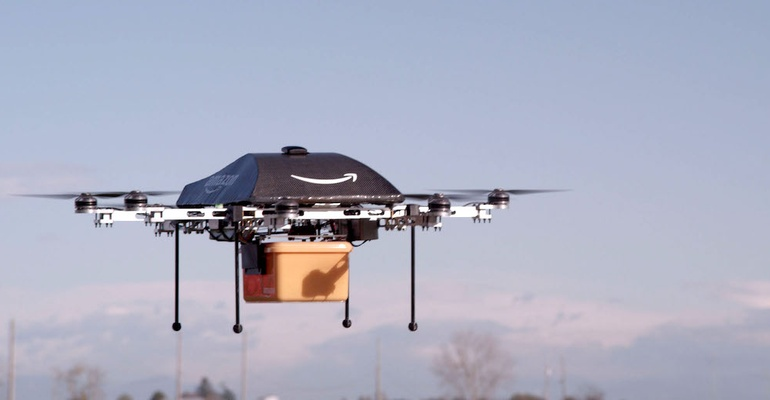
\includegraphics[scale=0.4]{images/prime.jpg}
    \caption{Amazon Prime Air drón}
    \label{fig:prime}
\end{figure}

Először 2016-ban próbálták ki, azóta még nem sikerült bevezetni különböző jogi korlátozások miatt. Olyan jogi elvárásoknak kell megfelelni, mint hogy:
\begin{itemize}
    \item Muszáj egy drón pilótának ellenőrizni a repülést és szükség esetén kötelező közbeavatkoznia.
    \item Egy ilyen pilóta csak 1 drónt felügyelhet egyszerre, kivéve ha rendelkezik megfelelő engedéllyel.
    \item A drónokat nem lehet közvetlen egy személy vagy gépjármű fellett működtetni.
    \item Problémát jelent továbba hogy nem minden légtér megfelelő a drónokkal való szállításra. A reptér mellett fekvő nagyvárosokban például biztos hogy nem lehet drónokkal szállítani.
    \item A csomagot szállító drónnak is kell rendelkeznie engedéllyel, hogy alkalmas kereskedelmi szállításra.
\end{itemize}

Az FAA 2020-ban engedélyezte az Amazonnak a drónokkal való csomagszállítást, de egyelőre csak tesztelik a technológiát pár városban.\\
Az Amazon felhőszolgáltásai között is található olyan szolgáltatás amellyel könnyedén kezelhetjük az IoT eszközöket, jelen esetben a drónokat.
Ilyen az IoT Core vagy az IoT Things Graph amin grafikus felületen összeköthetjük és beállíthatjuk az eszközeink közti kommunikációt. \\
A DHL is próbálkozott hasonló csomagkézbesítő megoldásokkal, ők egy úgynevezett  Parcelcopter-el \ref{fig:parcelcopter} szállították a csomagokat.

\begin{figure}[h]
    \centering
    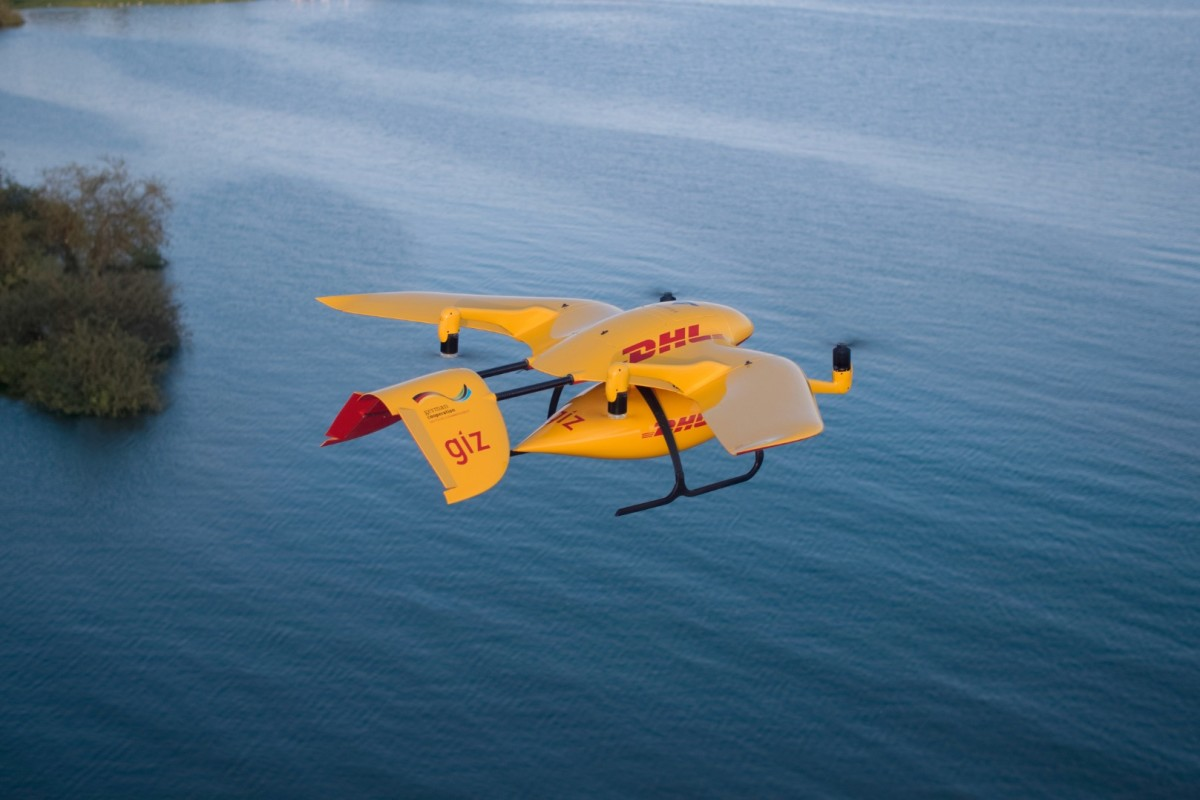
\includegraphics[scale=1.0]{images/parcelcopter.jpeg}
    \caption{DHL Parcelcopter V4.0}
    \label{fig:parcelcopter}
\end{figure}
Ám ők más problémát akarnak megoldani, a nagyon nehezen elérhető helyekre probálnak csomagokat szállítani.\\
A FlytBase \cite{flyt} vállalat már kínál szoftveres megoldásokat a automatizált drónok valós idejű figyelésére és irányítására, útvonal tervezésre valamint flotta menedzselésre.\\
A jövőben teljesen elképzelhető hogy a csomagok felét drónok szállítják ki. Csak az Amazon naponta átlagosan 7 mill3ió csomagot szállít ki,
és bevallásuk szerint a csomagok 86\%-a drónnal szállítható.

\Section{A szállítási probléma absztrakt modellje}

A szállítási modellünk alapvetően úgy nézne ki, hogy a raktár és a kiszállítási hely közti távolság függvényében a csomagokat a raktárból drónok, vagy drónokkal felszerelt teherautók viszik ki.
A teherautók a kiszállítási hely közelében használnák a drónokat hogy kézbesítsék a drónokat.\\
A drónok 3G, 4G vagy 5G hálózaton kommunikálnának az adatközpontokkal.\\
Az adott hálózaton elérhető sávszélesség függvényében a drónok változtathatják az elküldött adatok mennyiségét és a küldés ütemezését, gyakoriságát.\\
A drónok repülése előre megtervezett, minél hatékonyabb kell hogy legyen de valós időben kell reagálniuk a helyzetekre, problémákra.\\
A drónokból a szállítás során keletkező nagymennyiségű adatot az adatközpontoknak valós időben hibamentesen
és hatékonyan kell tudnia kezelni anomáliák nélkül. Ehhez nagyon fontos a terhelés megfelelő elosztása. \\

A drónok csomag szállítási folyamatáról a következőket feltételezzük:
\begin{itemize}
    \item Egy drón  véges akkumlátoridővel vagy üzemanyaggal rendelkezik és mindig vissza kell tudnia térnie egy töltőállomásra, amely lehet egy drónszállító teherautó vagy raktár.
    \item A csomag kézbesítés a csomag átvételére vonatkozó ideje elhanyagolható.
    \item Minden drón fel van szerelve megfelelő kommunikácós és helymeghatározó eszközökkel, valamint az kommunikál az adatközpontokkal.
    \item Feltételezzük hogy a drónok el vannak látva szenzorokkal hogy felismerjék az akadályokat és erről értesítsék az adatközpontokat.
\end{itemize}
A mi esetünkben csak akkumlátorral üzemelő drónok lesznek. Minden drón küld telemetria adatokat,
ebbe benne lesz az akkumlátor töltöttség százalékban, valamint az akkumlátor hőmérséklete is.
A drónok a telemetria adatok részeként küldenek helymeghatérozásra alkalmas
földrajzi szélesség, hosszúság koordinátákat és magasságot.
Továbbá kapunk még információkat a drón sebességéről,
gyorsulásáról, tájoló iránytűjének állásáról, motorjainak hőmérsékletéről,
mindezt egy időpecséttel megbélyegezve hogy az üzenetek elküldésének idejét is tudjuk.

% TODO: Ezek így szövegesen leírva stimmelnek, de érdemes lenne jelöléseket is rakni hozzá, hogy fel lehessen majd írni az optimalizálási feladatot belőle.
Hogy el tudjuk dönteni melyik drón hova tud a leghatékonyabban szállítani, a következő mennyiségeket jelölni kell. Hány km-re van a felszállási ponttól a csomag leadási helye (távolság km-ben),
mekkora akkumlátor töltöttséggel rendelkezik a drón (töltöttség százalékban), és a csomag súlya.
Ezekből a jelölésekből, ha tudjuk hány csomag rendelés és hány drón van, már fel tudjuk írni az optimalizálási feladatot.


\[
\begin{bmatrix}
    0.9 & 1 & 1 \\
    1 & 1.45 & 0.8\\
    1.32 & 1 & 0.8
\end{bmatrix}
\]
\Section{A szállítási probléma egy konkrét számítási példája}
% TODO: Készíteni kellene egy sematikus ábrát, amin egy szállítási állapot, gráfos formában megadott probléma látható.

\Section{A Go nyelv áttekintése }

A Go program nyelv, (sokszor Golangként emlegetik) egy nyílt forráskódú modern programozási nyelv melyet a Google fejlesztett ki.\\
A Google-nél olyan problémák adódtak, hogy a konkurrenciát nem tudták megfelelően kezelni a még eredetileg
1 processzoros számítógépekre kifejlesztett nyelvek, mint a Java, C++.
Persze azóta sokat fejlődött ezen nyelvek konkurrenciakezelése de nem tudnak versenyezni a Go-val
ha a gépi és fejlesztői hatékonyságot is figyelembe vesszük.
Probléma volt az is, hogy ezeknek a nyelveknek nagyon nagy a fordítási idejük. A 2000-es évek végén ez azt jelentette
hogy egy Java vagy C++ program a Google-nél 1 hét alatt fordult le, csak hogy ki tudják próbálni.
A nyelvek bonyolultságával is baj volt, ahogy fejlődtek a nyelvek egyre nehezebb volt egy régi programot tovább fejleszteni,
illetve új programozóknak megtanulni a nyelvet.\\
Hogy ezeket a problémákat orvosolják, a Google a legjobb tervezőket hívta össze, hogy megalkossák a Go nyelvet.
A fejlesztést olyan szakemberek vezették, akik korábban a Unix operációs rendszer, a Java HotSpot JVM
vagy az UTF-8 karakterkódolás fejlesztésében is kulcsszerepet játszottak.
Például Ken Thompson, Rob Pike és Robert Griesemer.\\
A cél az volt, hogy régebbi általános célú nyelvek hiányosságait kiküszöböljék, és csökkentsék a bonyolultságot, hiszen a megváltozott üzleti és technológiai körülmények
között ezek a nyelvek nem bizonyultak elég hatékonynak.
Nem várhatták el hogy egy friss diplomás hatékonyan kezeljen egy olyan ''felpuffadt'' nyelvet mint a Java.\\
A felhőben való futtatásra olyan alkalmazások készítésére volt igény, amelyek nagy hatékonysággal futnak és kiválóan skálázódnak.
A végeredmény egy olyan nyelv amely általános célú, könnyen tanulható, kifejező, tömör, letisztult és hatékony.
Éppen ezért kiválóan alkalmazható ott, ahol a kódbázishoz nagyszámú, gyakran cserélődő, változó összetételű programozói gárda fér hozzá,
akár időben és földrajzi elhelyezkedésben is megosztva.\\
Szintaktikailag a C-hez hasonlít de nagyon könnyen tanulható nyelv.
A legnagyobb újítás a konkurrencia mechanizmus (főleg a saját ütemező) és hibakezelés volt.
A Go konkurrencia mechanizmusa megkönnyíti olyan programok írását amelyet a legtöbbet hozzák ki a többmagos és hálózaton összekötött gépekből.
Gyorsan lefordul gépi kódra de rendelkezik garbage collection-el és runtime reflection is van beépítve.
Gyors, statikus nyelv de úgy érezzük mintha egy dinamikus futás időben fordított nyelv lenne.
Tartalmaz \textit{race detector}-t is ami nagyon fontos egy ilyen nyelvben, mert fel tudja ismerni a konkurrens/párhuzamos programozásnál felmerülő gyakori problémákat.
Mivel nagyon jól kihasználja a gép erőforrásait és a hálózatot manapság a felhőben futó kódok nagyrésze Go.
Beszédes, hogy a Linux Foundation által létrehozott Cloud Native Computing Foundation (CNCF) keretein
belül támogatott projektek nagy része Go-ban íródott, többek között a Kubernetes, a Prometheus, az Istio, de ebben írták a Dockert is.\\

% TODO: Ide kellene hivatkozás.

\paragraph{A Go konkurrencia mechanizmusa} \mbox{} \\
A konkurrencia a nyelv alapjának része. A 3 legfontosab dolog ebből a szempontból az hogy a Go-nak saját ütemezője van,
a gorutinok (''goroutine'') és csatornák (''channel'').\\
A saját ütemező (scheduler) sokkal hatékonyabb mintha csak létrehoznánk egy processzt és hagynánk hogy az OS ütemezze,
mivel így az ütemező meg tudja határozni hogy az adott gorution milyen állapotban van (várakozik, futtatható, vagy fut) és hatékonyabban tudja
kiosztani az erőforrásokat. Értelemszerűen például egy blokkoló, épp I/O műveletet végző gorutint nem fog futtatni hanem helyette más gorutinokat részesít
előnyben. De fontos hogy az ütemező nem determinisztikus, így nem tudjuk előre megmondani melyik gorutin fog következni.\\
4 féle esemény fordulhat elő a Go programokban ami miatt az ütemező döntéseket hozhat:
\begin{itemize}
    \item A \emph{go} kulcsszó használata
    \item Garbage collection
    \item Rendszer hívások
    \item Szinkronizálás és orchesztráció, vezérelés
\end{itemize}
A \emph{go} kulcsszó használata: \par
A go kulcsszó létrehoz egy új gorutint, így az ütemezőnek lehetősége van beavatkozni.\\
Szinkronizálás és vezérlés: \par
Ha egy atomi, mutex, vagy csatorna művelet, függvényhívás miatt egy Gorutin blokkolni fog, az ütemező kontextus cserével egy másik gorutinnak adhat erőforrást. Ha a blokkolt Gorutin újra futtathatóvá válik, sorba állítja az ütemező és végül visszakapja az erőforrást.\\

A gorutinok ugyanabban a címtérben futnak, ezért a megosztott memóriához való hozzáférést szinkronizálni kell.
A csatornák a típusos vezetékek amelyeken adatokat küldhetünk és fogadhatunk a csatorna operátorral, <-.
Az adatok a nyíl irányába folynak.
\begin{python}
    ch <- v    // Snd v to channel ch.
    v := <-ch  // Receive from ch, and
    // assign value to v.
\end{python}
Alapértelmezett beaállítás szerint a csatornák blokkolnak amíg az egyik oldal küld vagy fogad.
Ez lehetővé teszi a szinkrinizációt anélkül hogy zárakat vagy feltétel változókat hoznánk létre.

Bufferelt csatornák
\begin{python}
    ch := make(chan int, 100)
\end{python}

\paragraph{A Go hibakezelése} \mbox{} \\
A hibakezelés nagyban megváltozott azzal hogy a Go-ban nem try és catch blokkba zárjuk a hibára futható programkódot
hanem van egy beépített hiba típus, ami a függvények visszatérési értéke lehet. Fontos tudni, hogy a Go-ban egy függvény többféle
visszatérési értékkel rendelkezhet. Amit mi írunk programkódot, szinte minden függvényünk utolsó visszatérési értéke egy hiba típus lesz.
Csak az olyan atomi műveleteket végző függvényeknél nem szoktunk hiba típust használni ami biztos hogy nem fut hibára normális körülmények között.
\begin{python}
    func Open(name string) (file *File, err error)
\end{python}
A fenti függvény például egy Fájl típus pointerét és egy hiba típust ad vissza. Ha nem futott hibába a program, az err változó nil értéket kap.

Tehát egy hiba kezelése például így nézhet ki:
\begin{python}
    file, err := Open(''fajlnev'')
    if err != nil {
    log.Println(err)
    return 0, err
    }
\end{python}



Pár vállalat aki használja:
\begin{itemize}
    \item Google
    \item Uber
    \item Netflix
    \item Youtube
    \item Dropbox
    \item BBC
\end{itemize}

Az előnyökhöz persze hátrányok is tartoznak, az egyszerűség mellé nem férnek el a generikus függvények.
Maga a nyelv nem tartalmaz osztályokat, illetve nincs öröklődés.
Viszont az objektum orientált paradigmákat használja és így is kell benne programozni.
Tartalmaz interfészeket, a típusokhoz így a structhoz is tudunk hozzárendelni úgynevezett receiver függvényeket, amelyeket más nyelvekben metódusoknak nevezünk, mert a típus egy példányára tudjuk meghívni.

% TODO: Külön szakaszban érdemes lenne kifejteni, hogy a konkurrencia kezelése (az aktor modell) pontosan mit takar, és hogy valósul meg a nyelvben.
